\section{DRAMCmdState Struct Reference}
\label{structDRAMCmdState}\index{DRAMCmdState@{DRAMCmdState}}
{\tt \#include $<$cmd\_\-issuer.h$>$}

Collaboration diagram for DRAMCmdState:\nopagebreak
\begin{figure}[H]
\begin{center}
\leavevmode
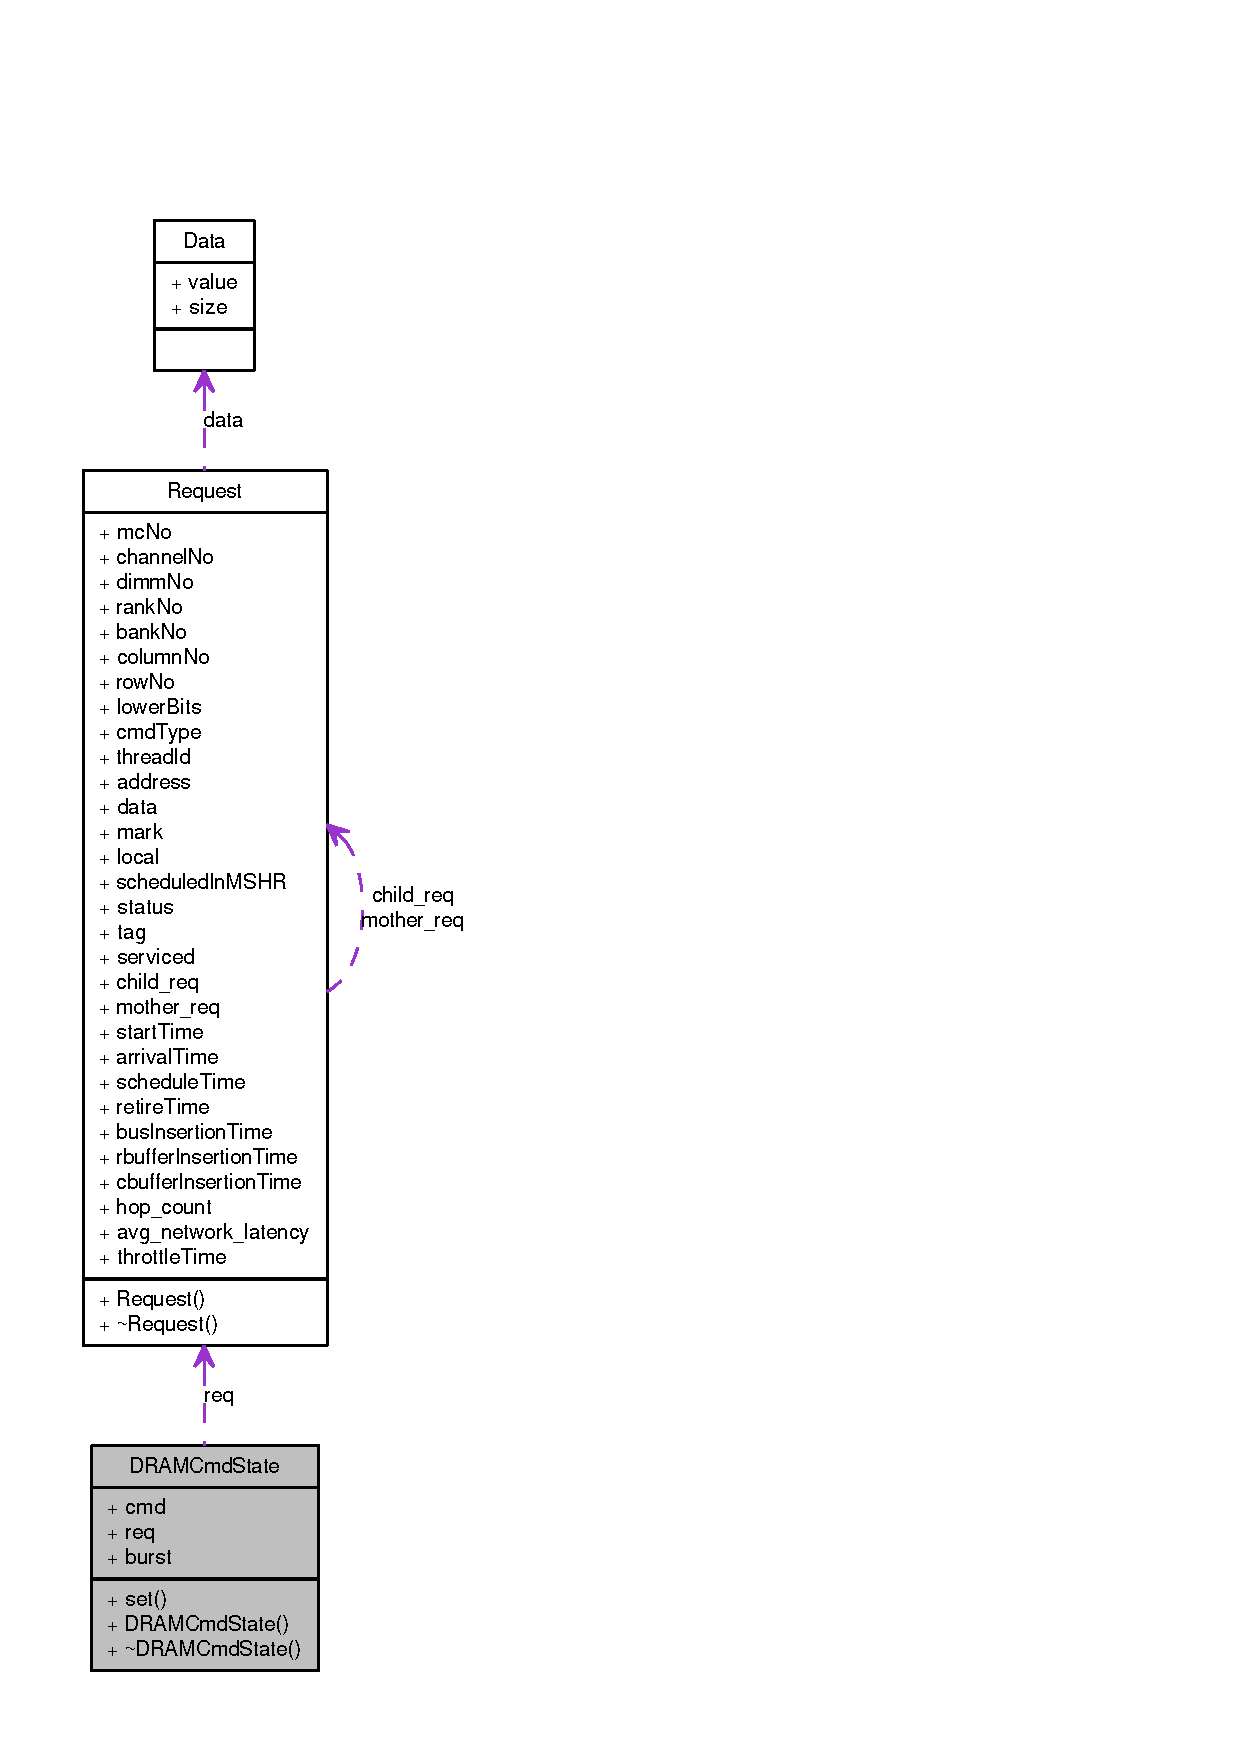
\includegraphics[height=400pt]{structDRAMCmdState__coll__graph}
\end{center}
\end{figure}
\subsection*{Public Member Functions}
\begin{CompactItemize}
\item 
void {\bf set} ({\bf DRAMCmd} cmdS, {\bf BurstLength} burstL, {\bf Request} reqI)
\item 
{\bf DRAMCmdState} ()
\item 
{\bf $\sim$DRAMCmdState} ()
\end{CompactItemize}
\subsection*{Public Attributes}
\begin{CompactItemize}
\item 
{\bf DRAMCmd} {\bf cmd}
\item 
{\bf Request} {\bf req}
\item 
{\bf BurstLength} {\bf burst}
\end{CompactItemize}


\subsection{Detailed Description}


Definition at line 44 of file cmd\_\-issuer.h.

\subsection{Constructor \& Destructor Documentation}
\index{DRAMCmdState@{DRAMCmdState}!DRAMCmdState@{DRAMCmdState}}
\index{DRAMCmdState@{DRAMCmdState}!DRAMCmdState@{DRAMCmdState}}
\subsubsection[{DRAMCmdState}]{\setlength{\rightskip}{0pt plus 5cm}DRAMCmdState::DRAMCmdState ()\hspace{0.3cm}{\tt  [inline]}}\label{structDRAMCmdState_940294d20ed946530cb2731041c78a40}




Definition at line 64 of file cmd\_\-issuer.h.

References burst, cmd, NORMAL, and PRECHARGE.\index{DRAMCmdState@{DRAMCmdState}!$\sim$DRAMCmdState@{$\sim$DRAMCmdState}}
\index{$\sim$DRAMCmdState@{$\sim$DRAMCmdState}!DRAMCmdState@{DRAMCmdState}}
\subsubsection[{$\sim$DRAMCmdState}]{\setlength{\rightskip}{0pt plus 5cm}DRAMCmdState::$\sim$DRAMCmdState ()\hspace{0.3cm}{\tt  [inline]}}\label{structDRAMCmdState_ad2f74b8d98b2ed4799d06fb137da995}




Definition at line 69 of file cmd\_\-issuer.h.

\subsection{Member Function Documentation}
\index{DRAMCmdState@{DRAMCmdState}!set@{set}}
\index{set@{set}!DRAMCmdState@{DRAMCmdState}}
\subsubsection[{set}]{\setlength{\rightskip}{0pt plus 5cm}void DRAMCmdState::set ({\bf DRAMCmd} {\em cmdS}, \/  {\bf BurstLength} {\em burstL}, \/  {\bf Request} {\em reqI})\hspace{0.3cm}{\tt  [inline]}}\label{structDRAMCmdState_901fee4ee232a13830c3705ab9c514cc}




TODO needs to set this 

Definition at line 49 of file cmd\_\-issuer.h.

References burst, cmd, Request::data, PREFETCH\_\-SIZE, PREFETCHL, READ\_\-SIZE, READL, req, Data::size, WRITE\_\-SIZE, WRITEBACK\_\-SIZE, WRITEBACKL, and WRITEL.

Referenced by CmdIssuer::CmdIssuer(), and BusHandler::LowLevelCmdGen().

Here is the caller graph for this function:\nopagebreak
\begin{figure}[H]
\begin{center}
\leavevmode
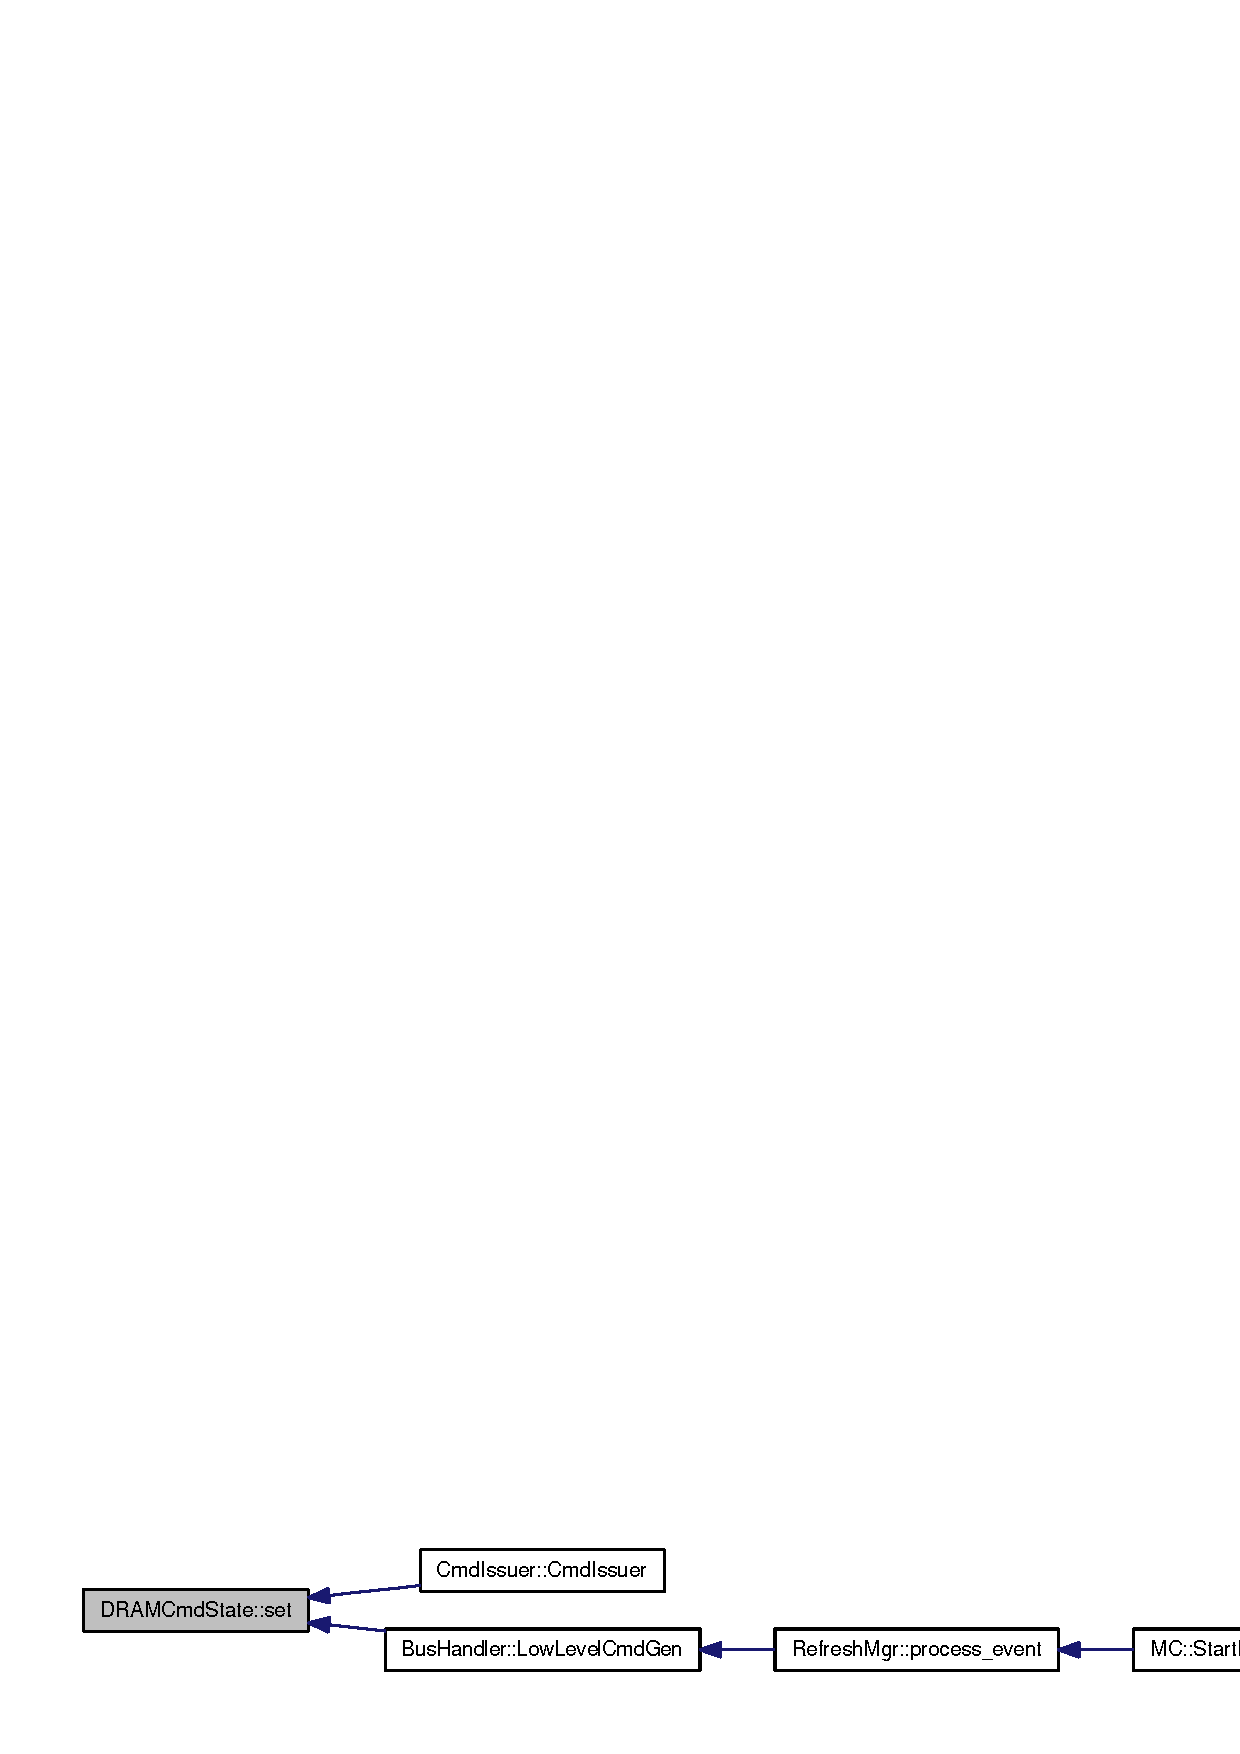
\includegraphics[width=401pt]{structDRAMCmdState_901fee4ee232a13830c3705ab9c514cc_icgraph}
\end{center}
\end{figure}


\subsection{Member Data Documentation}
\index{DRAMCmdState@{DRAMCmdState}!burst@{burst}}
\index{burst@{burst}!DRAMCmdState@{DRAMCmdState}}
\subsubsection[{burst}]{\setlength{\rightskip}{0pt plus 5cm}{\bf BurstLength} {\bf DRAMCmdState::burst}}\label{structDRAMCmdState_8b364745bf88499975f408a3d48293ff}




Definition at line 48 of file cmd\_\-issuer.h.

Referenced by CmdIssuer::CalculateBurstL(), DRAMCmdState(), and set().\index{DRAMCmdState@{DRAMCmdState}!cmd@{cmd}}
\index{cmd@{cmd}!DRAMCmdState@{DRAMCmdState}}
\subsubsection[{cmd}]{\setlength{\rightskip}{0pt plus 5cm}{\bf DRAMCmd} {\bf DRAMCmdState::cmd}}\label{structDRAMCmdState_29d74daa51471e7181215b381e013e9e}




Definition at line 46 of file cmd\_\-issuer.h.

Referenced by CmdIssuer::BankNotBusy(), CmdIssuer::BusNotBusy(), CmdIssuer::CalculateDataDelay(), CmdIssuer::CanSchedule(), DRAMCmdState(), DRAMChannel::process\_\-event(), CmdIssuer::process\_\-event(), set(), CmdIssuer::SetBusBusyTime(), and CmdIssuer::SetPrevState().\index{DRAMCmdState@{DRAMCmdState}!req@{req}}
\index{req@{req}!DRAMCmdState@{DRAMCmdState}}
\subsubsection[{req}]{\setlength{\rightskip}{0pt plus 5cm}{\bf Request} {\bf DRAMCmdState::req}}\label{structDRAMCmdState_73c981a3f268676ad91084cd9d01e262}




Definition at line 47 of file cmd\_\-issuer.h.

Referenced by CmdIssuer::BankNotBusy(), CmdIssuer::BanksFirstReq(), CmdIssuer::CanSchedule(), ResponseHandler::process\_\-event(), DRAMChannel::process\_\-event(), DataBusHandler::process\_\-event(), CmdIssuer::process\_\-event(), ResponseHandler::SearchBuffer(), set(), and CmdIssuer::SetPrevState().

The documentation for this struct was generated from the following file:\begin{CompactItemize}
\item 
{\bf cmd\_\-issuer.h}\end{CompactItemize}
